\documentclass[12pt]{beamer}
\usepackage[utf8]{inputenc}
\usepackage[slovene]{babel}
\usepackage{pgfpages}
\setbeamertemplate{note page}{\pagecolor{yellow!25}\insertnote}
\usepackage{palatino} % "Lep živahen" font
\setbeameroption{show notes on second screen=right}
\title{Monty Hall problem}
\author{Matej Neumann}
\institute{Univerza v Ljubljani}
\date{}
\beamertemplatenavigationsymbolsempty

\begin{document}

\begin{frame}
  \titlepage
\end{frame}

\begin{frame}
\begin{figure}
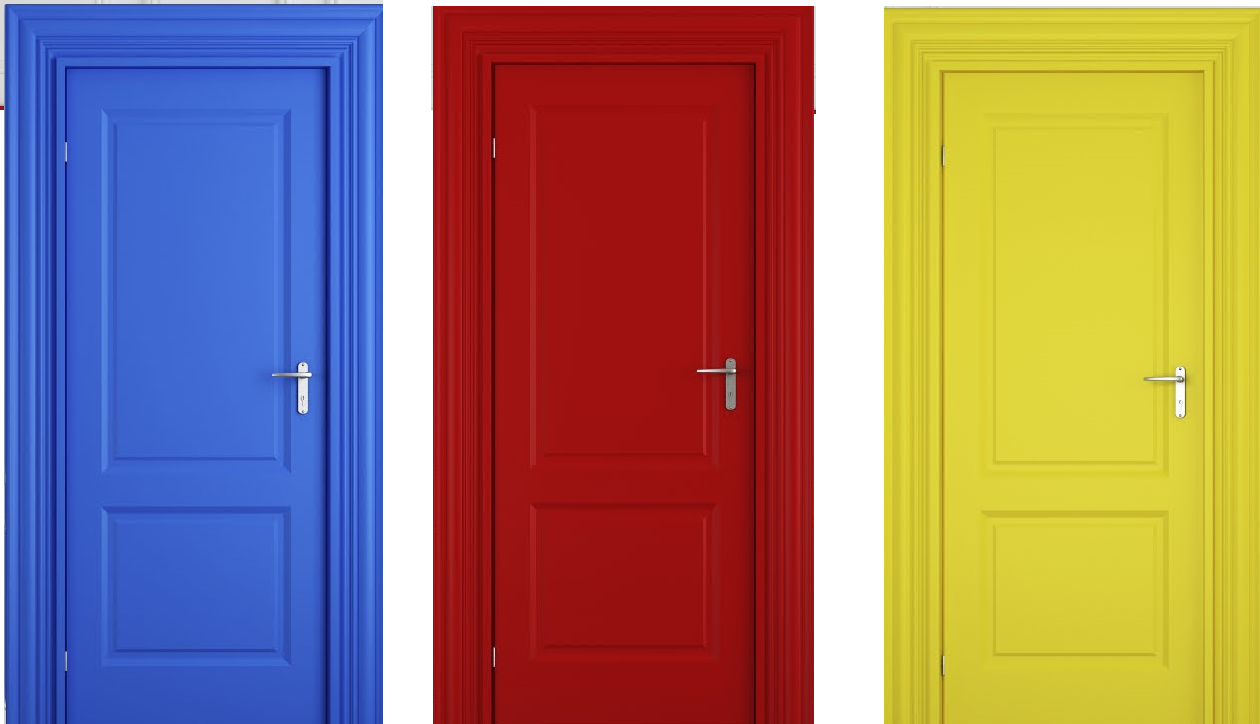
\includegraphics[width=\textwidth]{Zarta_Vrata_brez.png}

\end{figure}
\note{Začnimo najprej s vprašanjem. Pred vami so postavljena 3 vrata. Za enimi je nagrada ki jo želite (npr. lep nov avto). Za drugima dvema pa stojita dve kozi. Izberite ena vrata. Sedaj bom jaz odprl eno izmed preostalih dveh vrat za katerima stoji koza. Kolikšna je verjetnost da je avto  za vašimi vrati ? Pravilni odgovor je 1/3 }
\end{frame}

\begin{frame}
  \begin{figure}
  
\includegraphics[width=\textwidth]{LetsMakeADeal.jpg}

  \end{figure}

\end{frame}

\end{document}
